\documentclass{beamer}

% Información de la presentación
\title{Programación de Servicios y Procesos}
\subtitle{Introducción a la Asignatura}
\author{Prof. Víctor de Juan Sanz}
\institute{Colegio Santo Domingo Savio}
\date{\today}

\usepackage[utf8]{inputenc}

\usepackage{beamerthemeWarsaw}
\usepackage{longtable}

\usepackage{tcolorbox}
\usepackage{xcolor}


% Definir un nuevo comando para resaltar código al estilo Notion
\newtcolorbox{notioncode}{
  colback=gray!10,   % Fondo ligeramente gris
  colframe=gray!80,  % Borde gris oscuro
  sharp corners,     % Esquinas rectas (puedes cambiarlo a 'rounded corners' si prefieres)
  boxrule=0.5pt,     % Grosor del borde
  left=1mm,          % Espaciado interno a la izquierda
  right=1mm,         % Espaciado interno a la derecha
  top=1mm,           % Espaciado interno en la parte superior
  bottom=1mm,        % Espaciado interno en la parte inferior
  fontupper=\ttfamily,  % Tipo de letra monoespaciada (como el código)
  breakable          % Permitir que el bloque de código se divida entre páginas
}


% Definir un nuevo comando para resaltar código inline
\newcommand{\code}[1]{%
  \colorbox{gray!10}{\texttt{#1}}%
}

% Tema de la presentación (opcional)
\usetheme{Berlin} % Puedes cambiar Madrid por otro tema, como: Berlin, Warsaw, etc.

% Inicio del documento
\begin{document}

% Título de la presentación
\begin{frame}
    \titlepage
\end{frame}

% Tabla de contenidos
\begin{frame}{Contenido}
    \tableofcontents
\end{frame}

% Sección 1
\section{Conceptos Previos}

\begin{frame}{Procesos}
    \begin{itemize}
        \item Es una \textbf{instancia} de un programa en ejecución.
        \item Es una \textbf{entidad dinámica}.
        \item Toda la información relativa a un proceso se guarda en un \textbf{PCB (Process Control Block)}.
        \item Se lanza un proceso por cada ejecución del programa, cada uno con su propio PCB.
        \item Un proceos puede crear nuevos procesos.
    \end{itemize}
\end{frame}


\begin{frame}{Ejecución de un programa}
    Se debe cargar en memoria y consume los siguientes recursos:
        \begin{itemize}
            \item Memoria: Debe cargarse en memoria el código del programa.
            \item CPU: Ejecuta el proceso creado tras cargar el programa en memoria.
            \item Dispositivos de Entrada/Salida (E/S), normalmente compartidos entre varios procesos.
        \end{itemize}
    
\end{frame}


\begin{frame}
  \begin{figure}
        \centering
        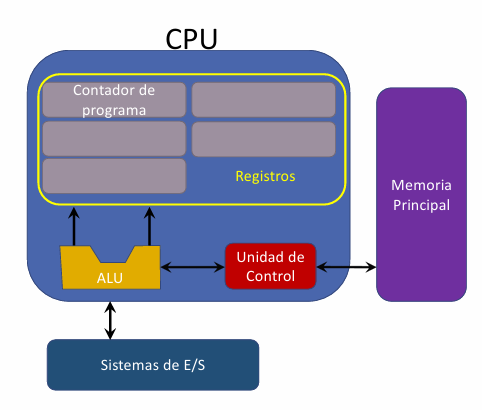
\includegraphics[width=0.75\linewidth]{img/cpu.png}
        \caption{Elementos de un procesador}
    \end{figure}

\end{frame}

\begin{frame}{PCB (Process Control Block)}
        \begin{itemize}
            \item PID (\textit{Process ID}).
            \item PPID (\textit{Parent PID}).
            \item Estado
            \item Contador de tiempo
            \item Priodidad
            \item Estado de E/S.
            \item Registros con "las variables del programa".
            \item ...
        \end{itemize}
    Cada proceso creado debe almacenar esta información.
\end{frame}

\section{Practicamos}
\begin{frame}{WSL}
    \begin{itemize}
        \item Abre powershell
        \item Ejecuta \code{wsl --install}
        \item Sigue los pasos de la instalación. Llama al usuario \textbf{cfgs} con contraseña \textbf{cfgs}.
        \item Disfruta de un linux instalado "nativo" dentro de Windows.
    \end{itemize}
\end{frame}

\begin{frame}{Practicamos}

Realiza los pasos en tu ordenador y realiza capturas de pantalla para guardarlo en tus apuntes. Deberás utilizar:
\begin{itemize}
    \item[UNIX] \code{pstree}, \code{ps -aF}, \code{top}
    \item[Windows] Administrador de tareas
    \item[Práctica] \begin{enumerate}
        \item Abre el mismo programa varias veces. Encuentra sus PIDs.
        \item Comprueba el árbol de jerarquías que te muestra \code{pstree}.
        \item ¿Cuál es el proceso que más tiempo lleva ejecutándose?
    \end{enumerate}
\end{itemize}



\end{frame}
% Sección 3
\section{Multitarea}

\begin{frame}{Monoprocesador}
    \begin{itemize}
        \item Ejecución simultánea de más de un proceso en un procesador durante un intervalo de tiempo.
        \item Actualmente los Sistemas Operativos, aunque se disponga de un solo procesador, permiten multitarea. ¿Cómo?
    \begin{itemize}
        \item   A intervalos regulares de tiempo
    \item   La ejecución del programa en curso se detiene.
    \item   Toma el control un programa “especial” del SO que puede parar la ejecución del proceso actual y hacer que pasa a ejecutarse otro proceso.
    \item   Este proceso es transparente al usuario del sistema.
    \item   En cada instante hay un único proceso en ejecución $\to$ Pero la rápida alternancia entre los procesos que van entrando en ejecución hace que el usuario no lo aprecie.
    \item   Por ello, se puede decir que en un determinado intervalo de tiempo múltiples procesos se ejecutan “simultáneamente”.
    \end{itemize}

\end{itemize}
\end{frame}

\begin{frame}{Monotarea}
  \begin{figure}
        \centering
        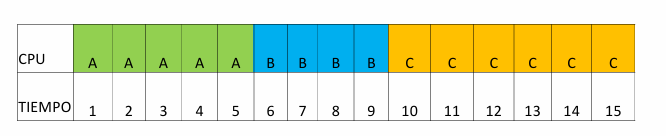
\includegraphics[width=0.7\linewidth]{img/Monotask.png} 
        \caption{Ejemplo de ejecución monotarea de 3 procesos.}
    \end{figure}

    \textit{Observa que, mientras se está ejecutando el proceso A parece que el C se ha "colgado" porque no puede ejecutar nada.}
\end{frame}

\begin{frame}{Multitarea}
  \begin{figure}
        \centering
        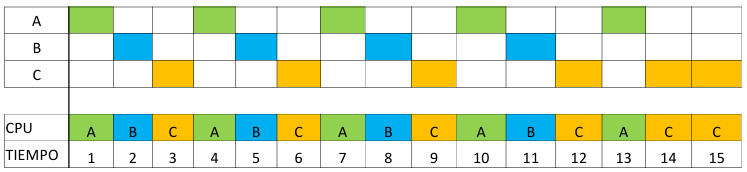
\includegraphics[width=0.7\linewidth]{img/Multitask_monoCPU.png} 
        \caption{Multitarea en un sistema monoprocesador.}
    \end{figure}

\begin{itemize}
    \item Eso sí, al cambiar de proceso en ejecución hay que realizar un \textbf{cambio de contexto:} almacenar el PCB del proceso que deja de ejecutarse para cargar el PCB del proceso que se va a ejecutar. 
    \item Hay que asegurarse que el programa sigue ejecutándose por donde iba.
\end{itemize}

\tiny{\textit{Disclaimer: Ejemplo meramente ilustrativo (no se tienen en cuenta distintos algoritmos de planificación, prioridades etc.) Simplemente consideramos round-robin con una “rodaja” de tiempo.}}
\end{frame}


% Conclusión
\begin{frame}{¿Compensa la multitarea-monoprocesador?}
\begin{itemize}
\item ¿A pesar de que al tiempo de ejecución del proceso hay que sumarle el tiempo del cambio de contexto y el de planificación de la ejecución de los distintos procesos por parte del Sistema Operativo? $\to$ SÍ!!!!!
\item Principales razones:
\begin{itemize}
\item El tiempo dedicado al cambio de contexto y planificación de la ejecución de los procesos es pequeño en comparación con el dedicado a la ejecución propiamente dicha de cada proceso.
\item Naturaleza del trabajo $\to$ En la actualidad el usuario realiza varias osas a la vez.
\item Uso del procesador $\to$ Durante la ejecución de un proceso hay periodos de tiempo bastante largos en los que no se hace uso del procesador (espera de finalización de operaciones de E/S principalmente) $\to$ Esos periodos se aprovechan para que otros procesos entren en ejecución.
\end{itemize}
\end{itemize}
\end{frame}

\section{Multiprocesador}

\begin{frame}{Multitarea multiproceso}
  \begin{figure}
        \centering
        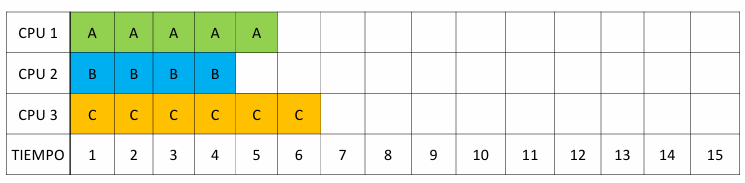
\includegraphics[width=0.7\linewidth]{img/Multitask_multiCPU.png} 
        \caption{Multitarea en un sistema multiprocesador.}
    \end{figure}
\end{frame}

\begin{frame}{Núcleos lógicos vs físicos - \textit{Hyperthreading}}
  \begin{figure}
        \centering
        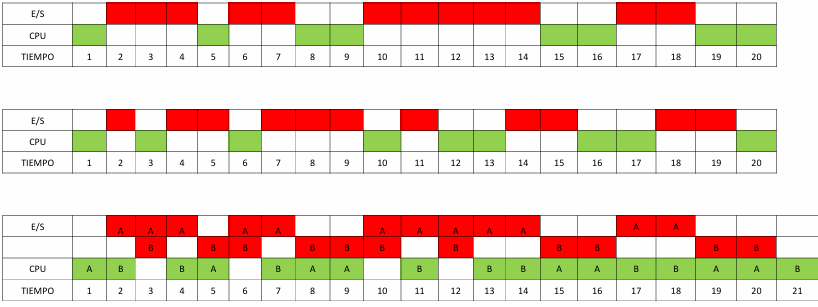
\includegraphics[width=0.7\linewidth]{img/Multitask_hyperthreading.png} 
        \caption{Un único procesador ejecutando en paralelo 2 proceso casi simultáneamente porque se optimizan las esperas de E/S.}
    \end{figure}
\end{frame}

\section{Estados de procesos}

\begin{frame}
  \begin{figure}
        \centering
        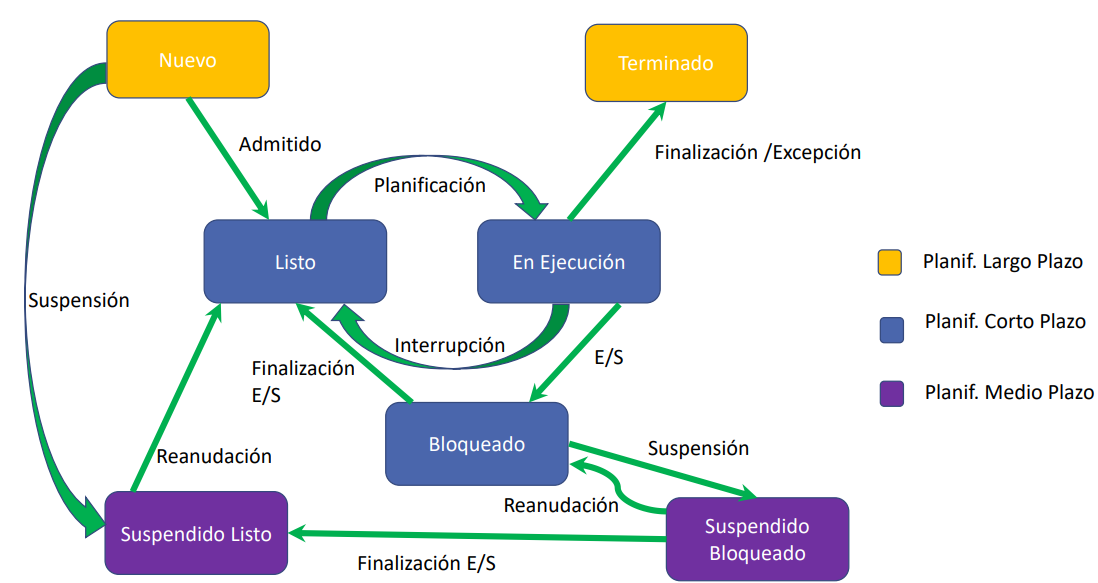
\includegraphics[width=0.95\linewidth]{img/estadosProceso.png} 
        \caption{Estados de un proceso.}
    \end{figure}
\end{frame}

\begin{frame}{Planificación a largo plazo}
    \begin{itemize}
        \item Se invoca de forma esporádica, generalmente cuando se inicia un nuevo proceso.
        \item Cambia el estado de los procesos de \textbf{nuevo} a \textbf{listo}, permitiendo que entren en la cola de procesos listos para ejecutarse.
        \item Regula el nivel de \textbf{multiprogramación}, decidiendo cuántos procesos pueden ser ejecutados simultáneamente.
        \item Mantiene un equilibrio entre procesos intensivos en CPU (\textit{CPU-bound}) y procesos intensivos en entrada/salida (\textit{I/O-bound}).
    \end{itemize}

\end{frame}

\begin{frame}{Planificación a medio plazo}
        \begin{itemize}
        \item Se invoca con menor frecuencia que el planificador a corto plazo.
        \item Decide si un proceso activo debe ser suspendido (swap-out) o si uno suspendido debe ser reanudado (swap-in).
        \item Ayuda a gestionar el uso de la memoria del sistema y evita que el sistema entre en un estado de sobrecarga (thrashing).
        \item Controla el nivel de \textbf{multiprogramación}, es decir, cuántos procesos están en memoria principal a la vez.
        \textbf{Gestiona el paso de procesos de memoria principal a secundaria} (suspensión) y viceversa (reanudación).
        \item Procesador solo puede acceder directamente a memoria principal.
        \item SWAP $\to$ Intercambio entre memoria principal y secundaria.
    \end{itemize}
\end{frame}


\begin{frame}{Planificación a corto plazo}

    \begin{itemize}
        \item Opera con alta frecuencia, tomando decisiones en cuestión de milisegundos.
        \item Cambia el estado de un proceso de \textbf{listo} a \textbf{ejecución}.
        \item Utiliza diferentes algoritmos de planificación, como \textit{Round Robin} (RR), \textit{First-Come, First-Served} (FCFS) y \textit{Shortest Job Next} (SJN).
        \item Tiene como objetivo maximizar el uso de la CPU, reducir los tiempos de espera y mejorar el tiempo de respuesta.
        \item Planificador a corto plazo realiza interrupciones periódicas $\to$ El sistema operativo ejecuta una rutina de gestión de interrupción y decide si se sigue ejecutando el proceso o hay que pasar a ejecutar otro.

    \end{itemize}
\end{frame}

 \begin{frame}{Resumen}
    \scriptsize
    \begin{longtable}{| p{1.5cm} | p{2.5cm} | p{1.5cm} | p{3cm} |}
        \hline
        \textbf{Planificador} & \textbf{Labor} & \textbf{Frecuencia} & \textbf{Objetivos} \\ \hline
        \textbf{Corto plazo} & Selecciona qué proceso listo será ejecutado por la CPU. Cambia el estado de \textit{listo} a \textit{ejecución}. & Alta (varias veces por segundo) & Maximizar el uso de la CPU, reducir el tiempo de espera, mejorar el tiempo de respuesta. \\ \hline
        \textbf{Medio plazo} & Suspende (swap-out) o reanuda (swap-in) procesos para gestionar la memoria y evitar sobrecarga. & Media (cuando sea necesario ajustar el uso de memoria) & Controlar el nivel de multiprogramación y gestionar la memoria de forma eficiente. \\ \hline
        \textbf{Largo plazo} & Decide cuántos y qué procesos serán admitidos al sistema, regulando la multiprogramación. & Baja (cuando se inician nuevos procesos) & Mantener el equilibrio entre procesos CPU-bound e I/O-bound, controlar el nivel de multiprogramación. \\ \hline
        \end{longtable}
    
\end{frame}

\end{document}
